\documentclass{article}
\usepackage{tikz}
\usetikzlibrary{shapes.geometric, arrows, positioning}

% Define colors
\definecolor{color1}{RGB}{250, 159, 0} % light orange
\definecolor{color2}{RGB}{86, 180, 233} % light blue
\definecolor{color3}{RGB}{204, 121, 167} % pink
\definecolor{color4}{RGB}{0, 158, 115} % green
\definecolor{color5}{RGB}{0, 114, 178} % dark blue
\definecolor{color6}{RGB}{213, 94, 0} % dark orange
\definecolor{color7}{RGB}{240, 228, 66}
\definecolor{colorblack}{RGB}{0, 0, 0}          % black

% Define block styles
\tikzstyle{startstop} = [rectangle, rounded corners, minimum width=3cm, minimum height=1cm, text centered, draw=black, fill=color1!50] %Represents the initialization or entry point of the program.
\tikzstyle{inputoutput} = [trapezium, trapezium left angle=75, trapezium right angle=105, minimum width=3cm, minimum height=1cm, text centered, draw=black, fill=color2!50]
\tikzstyle{module} = [rectangle, minimum width=3cm, minimum height=1cm, text centered, draw=black, fill=color3!20] %A Python module
\tikzstyle{class} = [rectangle, minimum width=3cm, minimum height=1cm, text centered, draw=black, fill=color3!50] %A Python class inside a module
\tikzstyle{function} = [rectangle, minimum width=3cm, minimum height=1cm, text centered, draw=black, fill=color5!50]  %These are methods or functions inside the classes.
\tikzstyle{decision} = [diamond, minimum width=3cm, minimum height=1cm, text centered, draw=black, fill=color6!50] %Conditional logic (e.g. if statements) inside a method or class, e.g., a branching logic.
\tikzstyle{external} = [rectangle, dashed, minimum width=3cm, minimum height=1cm, text centered, draw=black, fill=colorblack!50] %An optional, external Python package that a module might import, shown with a dashed arrow.

\tikzstyle{arrow} = [thick,->,>=stealth] %flow between modules, classes, and functions within the package
\tikzstyle{dashedarrow} = [thick,dashed,->,>=stealth] %optional or external dependencies

\begin{document}

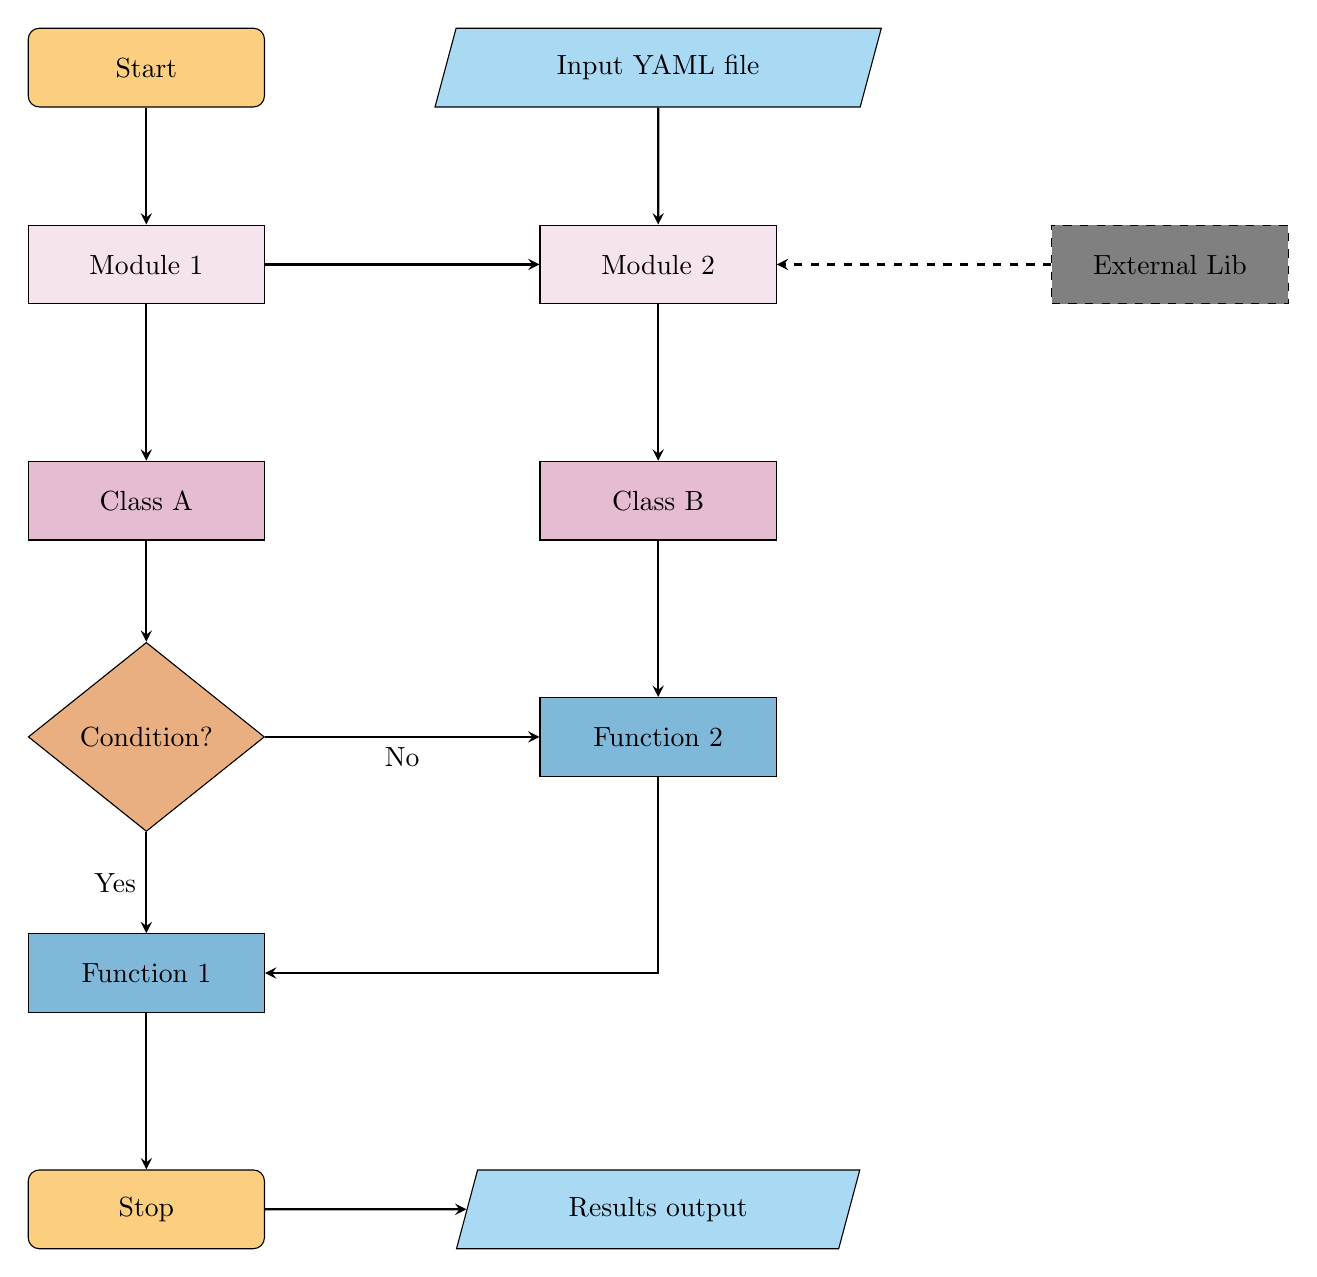
\begin{tikzpicture}[node distance=2.5cm]

% Nodes
\node (start) [startstop] {Start};
\node (module1) [module, below of=start] {Module 1};
\node (classA) [class, below of=module1, yshift=-0.5cm] {Class A};
\node (decision1) [decision, below of=classA, yshift=-0.5cm] {Condition?};
\node (function1) [function, below of=decision1, yshift=-0.5cm] {Function 1};
\node (module2) [module, right of=module1, xshift=4cm] {Module 2};
\node (input) [inputoutput, above of=module2] {Input YAML file};
\node (classB) [class, below of=module2, yshift=-0.5cm] {Class B};
\node (function2) [function, below of=classB, yshift=-0.5cm] {Function 2};
\node (external) [external, right of=module2, xshift=4cm] {External Lib};
\node (stop) [startstop, below of=function1, yshift=-0.5cm] {Stop};
\node (output) [inputoutput, right of=stop, xshift=4cm] {Results output};

% Arrows (solid for internal dependencies)
\draw [arrow] (start) -- (module1);
\draw [arrow] (module1) -- (classA);
\draw [arrow] (classA) -- (decision1);
\draw [arrow] (decision1) -- node[anchor=east] {Yes} (function1);
\draw [arrow] (decision1) -- node[anchor=north] {No} (function2);
\draw [arrow] (function1) -- (stop);
\draw [arrow] (input) -- (module2);
\draw [arrow] (stop) -- (output);

% Arrows for other modules and classes
\draw [arrow] (module1) -- (module2);
\draw [arrow] (module2) -- (classB);
\draw [arrow] (classB) -- (function2);

% Dashed arrow to indicate external dependency
\draw [dashedarrow] (external) -- (module2);

% Additional arrow to show cross-module flow
\draw [arrow] (function2) |- (function1);

\end{tikzpicture}

\end{document}
